
\subsection{Compiling to C}

	Due to the factors cited above for the deviation of Python memory
	and execution time from any theoretical estimates, 
	several of the core components (integrators, mass models, coupling
	functions) have been targeted towards a C source code backend, which has
	allowed for the compilation of simulations to native code loaded 
	either as a shared library accessed via the \texttt{ctypes} modules
	or as CUDA kernels accessed via the PyCUDA \cite{PyCUDA}.
	While such an approach may provide speed ups, they depend on the
	presence of a C compiler and, in the case of GPU, the CUDA toolkit and
	a compatible graphics card, and in the future, prepackaged versions of TVB
	will include precompiled objects for most kinds of simulations. 

	The approach used in compiling a simulation to native code takes advantage
	of the fact that CUDA is quite similar to C, and thus a generic template
	abstracts much of the boilerplate between the two. For each part of the 
	simulator, a generic function is customized with a class specific kernel;
	for example, in the case of a neural mass model, we have in the Python class

	\begin{lstlisting}
	class Generic2dOscillator(Model):
	    tau = FloatArray(...)
	    # etc.

	    device_info = model_device_info(
		pars=[tau, a, b, c, d, I],
		kernel="""
		float tau  = P(0)
		    , a    = P(1) ; // etc

		// state variables
		    , v    = X(0)
		    , w    = X(1)

		// aux variables
		    , c_0  = I(0)   ;

		// derivatives
		DX(0) = d * 
		(tau * (w - v*v*v + 3.0*v*v + I + c_0));
		DX(1) = d * 
		((a + b*v + c*v*v - w) / tau);
		"""
	    )
	\end{lstlisting}

	\noindent where the device\_info attribute is used to specify how the
	class's mathematical description fits into the general model function:

	\begin{lstlisting}
	/* wrapper for model specific code computing RHSs of diff-eqs */
	__device__
	void model_dfun(
	  float * _dx, float *_x, float *mmpr, float *input)
	{
	#define X(i) _x[n_thr*i]
	#define DX(i) _dx[n_thr*i]
	#define P(i) mmpr[n_thr*i]
	#define I(i) input[i]

	    // begin model code
	    \$model_dfun
	    // end model specific code

	#undef X
	#undef DX
	#undef P
	#undef I
	\end{lstlisting}

	\noindent where the C preprocessor defines allow the model specific
	kernel to easily reference the correct parts of the multidimensional 
	per-thread arrays (in the case of the GPU). 

	 \begin{figure}
		{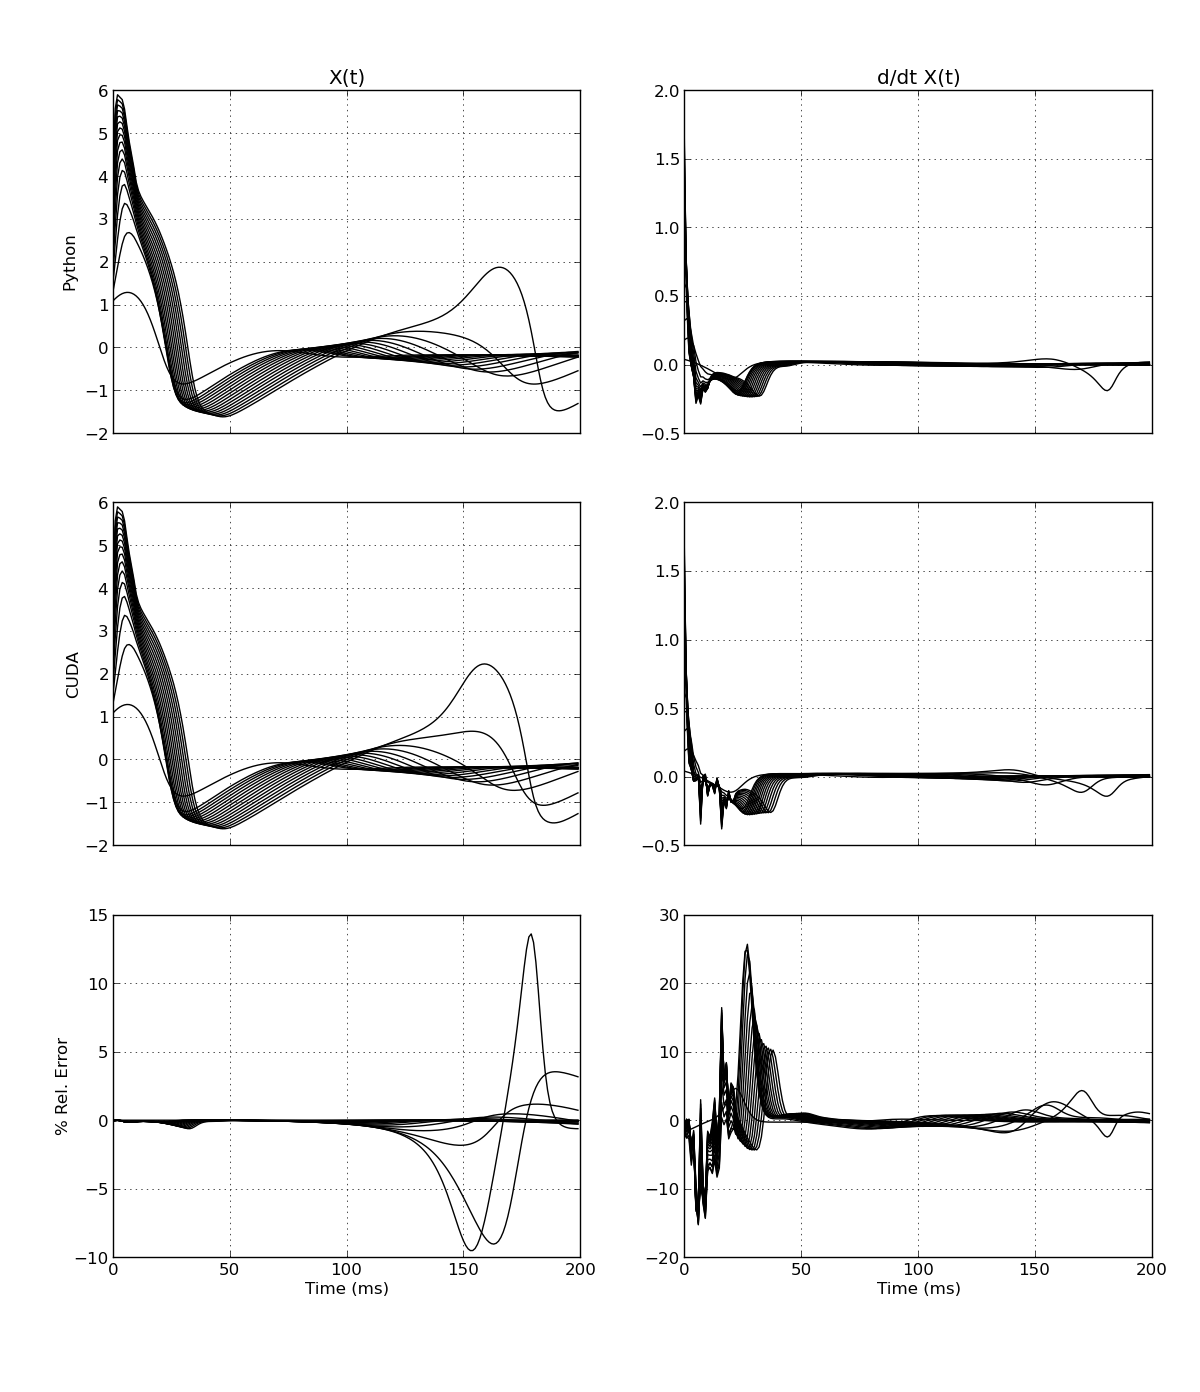
\includegraphics[width=0.48\textwidth]{images/gpu_dxdt.png}}
		\caption{
		Right A typical parameter space exploration, 32 x 32 grid of
		coupling strength (y-axis) v. neural excitability (x-axis).
		This grid of simulations was run on both TVB's Python/NumPy
		implementation and the new GPU backend for 200 ms simulation
		time with otherwise default parameters. The former took ~2
		hours and the latter ~ 1 min. Left Quantitative comparison of
		solutions and instantaneous derivatives is shown for an even
		sampling of the parameter space across k where a = -2, because
		this slice showed the most error on the GPU. 	
		}
		\label{fig:gpu_dxdt}
	\end{figure}

	 \begin{figure}
		{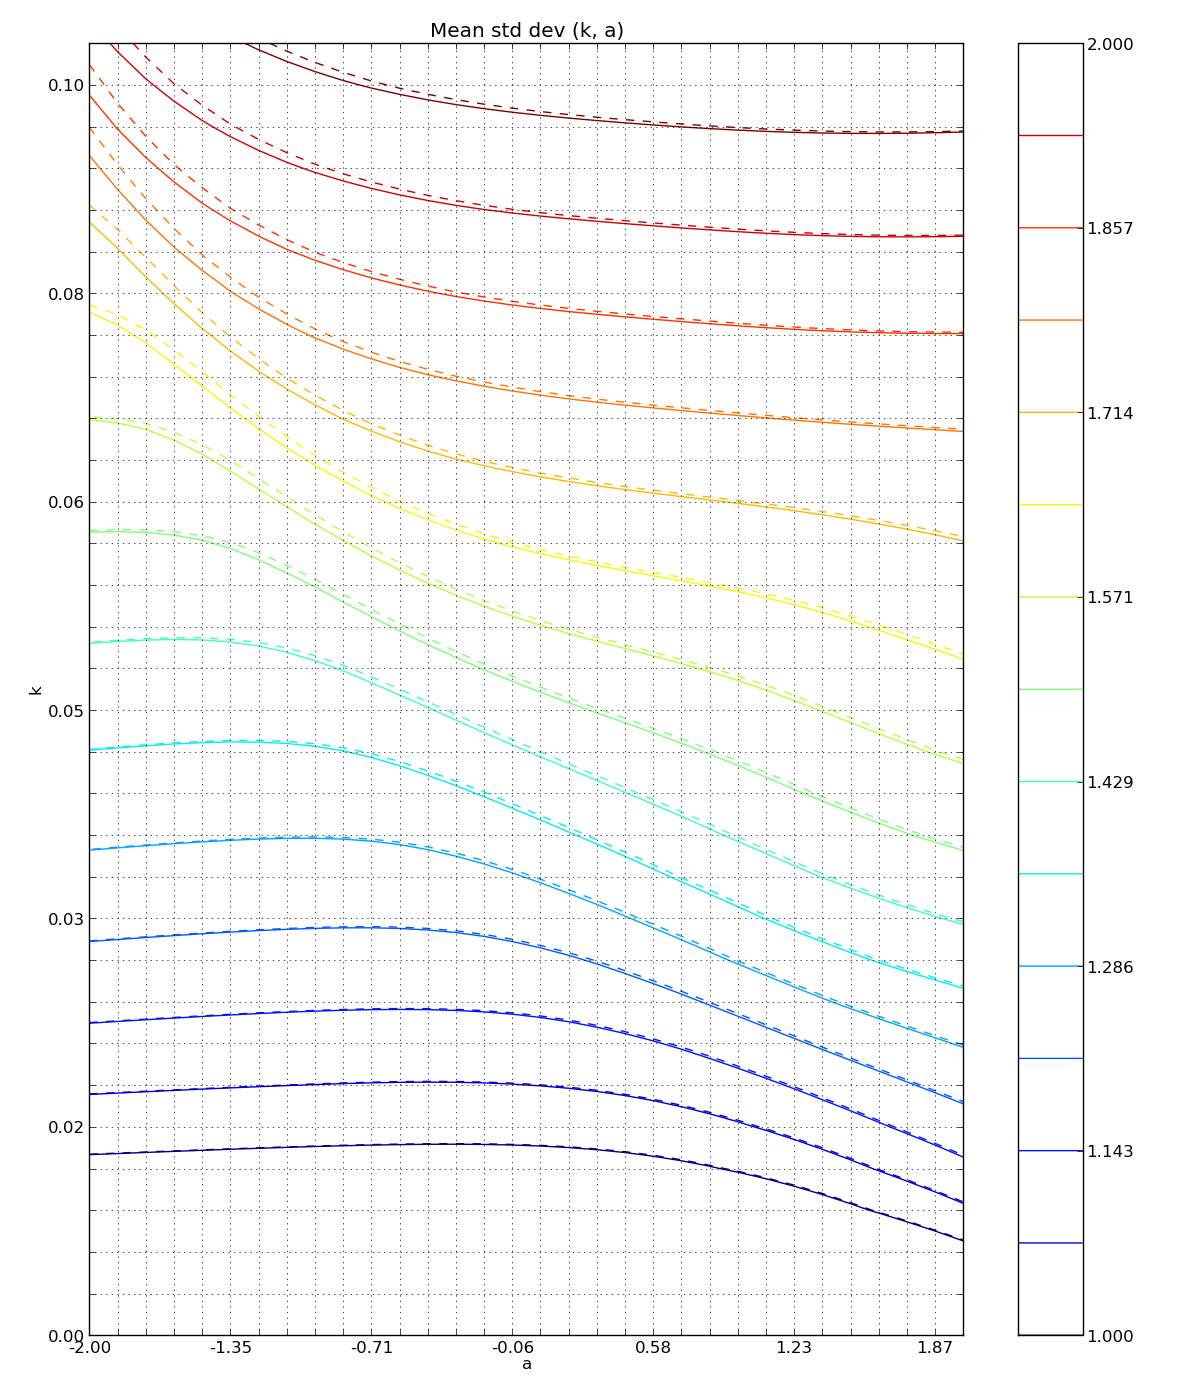
\includegraphics[width=0.48\textwidth]{images/gpu_pse.png}}
		\caption{}
		\label{fig:gpu_pse}
	\end{figure}

	\note[sk]{One figure or two, re captions}

	\note[sk]{Specify hardware (GPU/CPU) and whether Numpy is mkl-linked, to 
	    provide a more solid foundation for timing comparisons...}

	\note[sk]{It would be interesting to see a longer run (say a few seconds)
	    to show if/how-quickly the error grows...}

	As can be seen in the listing \note[sk]{can listings be numbered and labelled...}, the calculations
	in native code are performed with 32-bit floating point numbers, and it
	is reasonable to ask if this is numerically accurate. In Fig 
	\ref{fig:gpu_pse}, we present a parameter space exploration performed with
	both the pure Python NumPy simulator and the GPU simulator, showing the 
	isocontours of average standard deviation in the parameter space. Some
	deviation can be identified visually in parts of the parameter space, and
	in in Fig \ref{fig:gpu_dxdt}, we show in more detail time series of 
	the Python and GPU solutions.

	 \begin{figure}
		{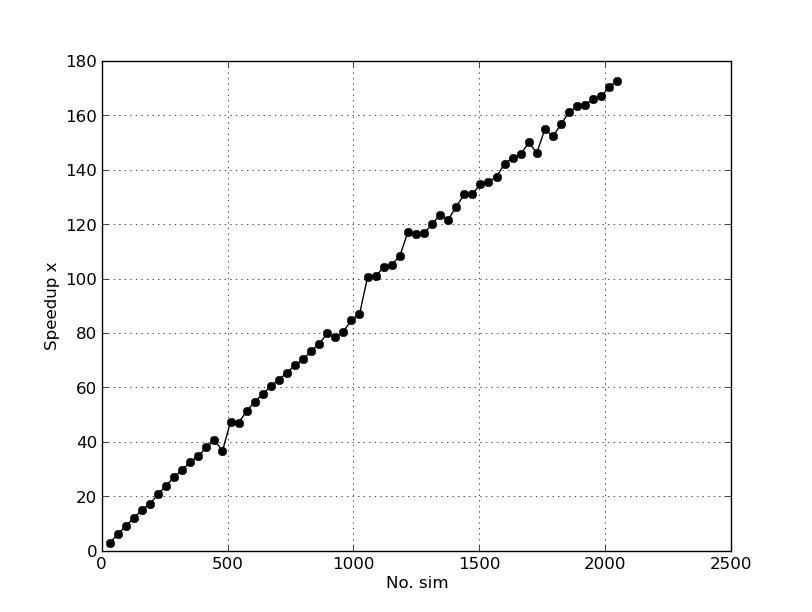
\includegraphics[width=0.48\textwidth]{images/gpu_acceleration.png}}
		\caption{}
		\label{fig:gpu_acceleration}
	\end{figure}

	This approach allows significant acceleration of parameter sweeps in the
	case of the GPU by taking
	advantage of the fact that in many cases, only numerical values vary
	between different threads and not memory access patterns. Where one of the
	dimensions of a parameter sweep implies changing memory access patterns, 
	for example conduction speed, it is advantageous to reorder the parameters,
	so that such memory varying parameters only change between grids of GPU
	threads and not within.

	In Fig \ref{fig:gpu_acceleration}, we plot the speedup brought by the GPU
	over the Python NumPy simulator as a function of the number of simulations 
	performed simulataneously on the GPU.



